\documentclass[12pt]{report}

\usepackage[a4paper]{geometry}
%\geometry{left=2.5cm,right=2.5cm,top=2.5cm,bottom=2.5cm, a4paper}
\usepackage[utf8]{inputenc}
\usepackage{amsmath}
\usepackage{amsthm}
\usepackage{amssymb}
\usepackage{ulem}
\usepackage{graphicx}
\usepackage{caption}
\graphicspath{}
\usepackage[document]{ragged2e}
\usepackage{setspace}
\usepackage{tabularx}
\usepackage[slovene]{babel}
\usepackage{textcomp, gensymb}
\usepackage{siunitx}
\usepackage{pdfrender,xcolor}
\usepackage{hyperref}
\usepackage{xurl}
\usepackage{float}
\usepackage{titlesec}

\newfloat{slika}{htbp}{loc}
\floatname{slika}{Slika}

\newfloat{tabela}{htbp}{loc}
\floatname{tabela}{Tabela}

\title{
  
\includegraphics[width=0.4\textwidth]{fmf_logo}\\
  {\small Oddelek za fiziko} \\
  {Meritve magnetnega polja z indukcijo }\\
  {\small Poročilo pri fizikalnem praktikumu III}\\

}
\date{}
\author{ avtor: Kristofer Č. Povšič \\[5 cm]
 \small  Asistentka: Jelena Vesić
}


\titleformat{\chapter}[hang]{\Huge\bfseries}{\thechapter{. }}{0pt}{\Huge\bfseries}

\setlength\parindent{0pt}

\begin{document}

\setcounter{page}{2}

\maketitle

\chapter*{Uvod}

Magnetno polje merimo z majhno tuljavico z veliko ovoji, ki je postavljena vzporedno zunanjemu magnetnemu polju. Napetost se v tuljavi inducira v dveh primerih: ob prekinitvi toka elektromagneta ali premiku tuljavice iz področja polja. 

Inducirano napetost $u$ izračunamo iz enačbe

\begin{equation}
  U = -\frac{\text{d}\phi}{\text{d}t} = - NS \frac{\text{d}B}{\text{d}t}\cos\alpha
\end{equation}

kjer je $\phi$ magnetni pretok, $N$ število ovojev, $S$ ploščina tuljavice, $B$ gostota magnetnega polja in $\alpha$ kot med osjo tuljavice in smerjo magnetnega polja. 

Pri indukciji napetosti U je navitje porazdeljeno med notranjim $r$ in zunanjim $R$ radijem: 

\begin{equation}
  \text{d}U = -\frac{\text{d}B}{\text{d}t}\pi r^2 \cos \alpha \text{d}N
\end{equation}

Gostota navitja $\text{d}N$ naj bo konstantna: 
\begin{equation}
  \frac{\text{d}N}{2 \pi r \text{d}r} = \frac{B}{\pi (R^2 - r^2)}
\end{equation}

Iz tega dobimo po integriranju v mejah med r in R: 

\begin{equation}
  U = - N\pi \frac{R^2 + r^2}{2} \frac{\text{d}B}{\text{d}t} \cos \alpha
\end{equation}

Inducirana napetost je sorazmerna s spremembo gostote magnetnega polja $\frac{\text{d}B}{\text{d}t}$. Zanima nas pa vrednost gostote magnetnega polja B. Na izhod priključimo integrator in dobimo 

\begin{equation}
  U_{iz} = \frac{N}{RC} \frac{R^2 + r^2}{2} \pi B_2
\end{equation}


\chapter*{Naloga}

\begin{enumerate}
  \item Izmeri odvisnost gostote magnetnega polja $B$ na osi tokovne zanke z oddaljenostjo od njenega središča
  \item Izmeri relacijo med jakostjo električne toka I in gostoto magnetnega polja $B$ v elektromagnetu. 
\end{enumerate}

\begingroup
\let\clearpage\relax

\chapter*{Potrebščine}
\begin{itemize}
  \item 2 merilni tuljavi z notranjim $2r = (18 \pm 0.1)mm$ in zunanjim premerom $2R = (23 \pm 0.5)mm$, $N_1 = 2000$, $N_2 = 200$
  \item integrator z $R= (10.0 \pm 0.5)k\omega$ in $C = (1.0 \pm 0.1)\mu F$
  \item voltmeter, ampermeter, šolski usmernik omejen na $6A$ toka, zaščita pred sunki 
  \item velika tuljava s premerom $2R_0 = (250 \pm 2) mm$, $N_3 = 200$ ovoji z navpičnim nosilcem za merilno tuljavico
  \item elektromagnet na lesenem nosilcu
\end{itemize}

\chapter*{Navodilo}
Veliko tuljavo priključimo na šolski usmernik s tokom $ I = 4A$. Merilno tuljavo z večjim št. navojen nataknemo na navpični nosilec in jo priključimo na integrator. Izhod integratorja povežemo z voltmetrom. Zaradi neidealnosti elektronskih elementov izhod integratorja "leze"  tudi kadar na vhodu pripeljemo ničlo. Lezenje vstavimo s primerno nastavitvijo potenciometra na integrator, ničlo pa nastavimo s tipko reset. Izmerimo gostoto magnetnega polja $B$ na osi krožnega tokovodnika (tuljave) kot funkcijo razdalje od središča. Dobljeno vrednost $B(h)$ narišemo na graf in jo primerjamo s teoretično krivuljo $B_{zanka}(h)$ za tokovno zanko radija $r_0$ po kateri teče tok $I_0$. 

Šolski usmernik zvećemo z elektromagnetom pritrjenim na leseno stojalo. Na integrator priključimo merilno tuljavo z manj navoji. Elektromagnet je sestavljen iz dveh isto orientiranih navitij na ogrodju z magnetno mehkega železa z režo med njima. V slednji sondiramo gostoto magnetnega polja. Z izmeničnim vlečenjem oz. potiskanjem tuljave v režo izmerimo odvisnost $B(I)$ v intervalu od $0$ do $5A$. Narišemo graf. Iz naklona premice izračunamo kolikšen naj bi bil $N/L$ dolge prazne tuljave, ki bi imela enako zvezo med B in I kot obravnan elektromagnet. 
\endgroup


\chapter*{Obdelava podatkov}

Za prvi del meritev sem dobil sledeče podatke: 


\begin{tabela}[H]
  \centering
  \[
  \begin{array}{|c|c|}\hline
    h [cm] & U [mV] \\ \hline
    5.00 &  180.00\\ 
    6.00 &  171.00\\
    7.00 &  168.00\\
    8.00 &  143.00\\
    9.00 &  125.00\\
   10.00 &  111.00\\
   11.00 &   97.00\\
   12.00 &   84.00\\
   13.00 &   76.00\\
   14.00 &   69.00\\
   15.00 &   63.00\\
   16.00 &   60.00\\
   17.00 &   59.00\\
   18.00 &   56.00\\
   19.00 &   53.00\\
   20.00 &   27.00\\
   25.00 &   13.00\\
   30.00 &    9.00\\
   35.00 &    3.00 \\ \hline
  \end{array}
  \]
\end{tabela}


Izrišem sledeč graf: 

\begin{slika}[H]
  \centering
  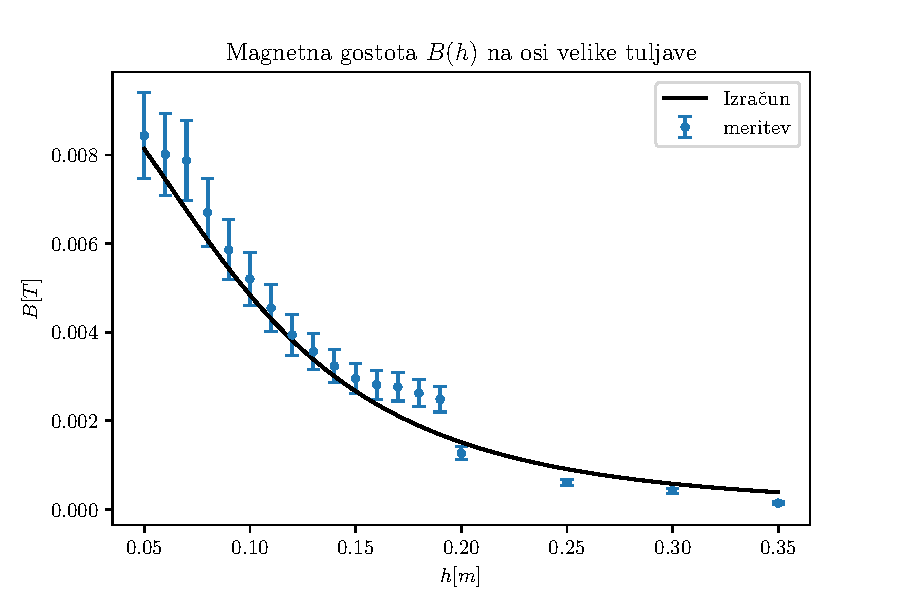
\includegraphics{graf1}
  \caption{\small Pričakovana ter izmerjena gostota magnetnega polja z napakami pri različnih oddaljenostih $h$ od središča velike tuljave}
\end{slika}

Za drugi del izmerim sledeče podatke: 


\begin{tabela}[H]
  \centering
  \[
  \begin{array}{|c|c|} \hline
    I[A] & U[mV] \\ \hline
    0.00 &    0.06\\
    0.50 &    0.60\\
    1.00 &    1.12\\
    1.55 &    1.54\\
    2.00 &    2.07\\
    2.52 &    2.50\\
    3.00 &    3.00\\
    3.50 &    3.45\\
    4.00 &    4.00\\
    4.50 &    4.35\\
    5.00 &    4.68 \\ \hline
  \end{array}  
  \]
\end{tabela}


Izrišem sledeč graf: 

\begin{slika}[H]
  \centering
  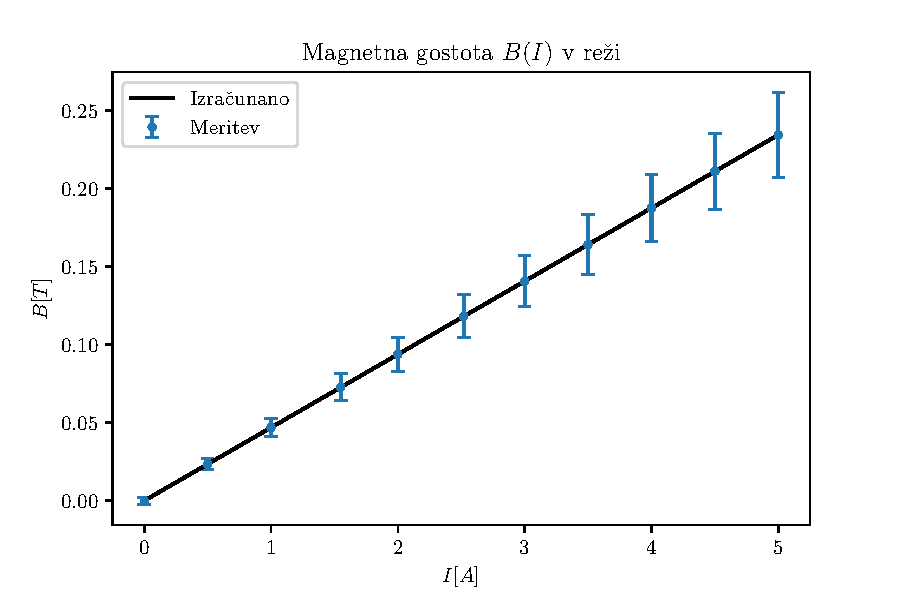
\includegraphics{graf2}
  \caption{\small Meritve magnetne gostote v reži elektromagneta pri različnih tokovih skozi elektromagnet z regresivno premico.}
  \label{fig:1}
\end{slika}

Na sliki \ref{fig:1} se jasno vidi linearna odvisnost. Naklon regresivne premice je: 

\[k = (0.047 \pm 0.008) \frac{T}{A}\]

Če bi torej elektromagnet pri enakem toku nadomestili z dolgo prazno tuljavo, bi potrebovali navitje gostote: 

\[ \frac{N}{L} = (110000 \pm 6000) m^{-1}\]

\end{document}